\tikzset{
  declare function={
    normpdf(\x,\mu,\sigma)=1/(\sigma * sqrt(2 * pi)) * exp(-((\x - \mu)^2)/(2 * \sigma^2));
  }
}
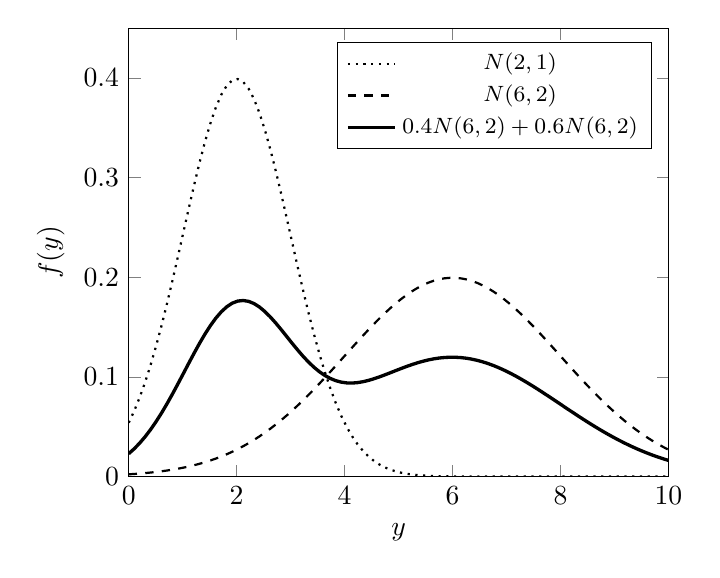
\begin{tikzpicture}
  \begin{axis}[
      samples=100, 
      domain=0:10, 
      xmin=0, 
      xmax=10, 
      ymin=0, 
      ymax=0.45, 
      xlabel={$y$}, 
      ylabel={$f(y)$}, 
      legend pos=north east
    ]
    \addplot[dotted, thick] {normpdf(x, 2, 1)};
    \addplot[dashed, thick] {normpdf(x, 6, 2)};
    \addplot[very thick] {0.4 * normpdf(x, 2, 1) + 0.6 * normpdf(x, 6, 2)};
    \addlegendentry{\footnotesize $N(2, 1)$};
    \addlegendentry{\footnotesize $N(6, 2)$};
    \addlegendentry{\footnotesize $0.4 N(6, 2) + 0.6 N(6, 2)$};
  \end{axis}
\end{tikzpicture}
